% =============================================================
%  Chapter 3 — Geometry-Only Structured Navigation:
%              The GRL-SNAM Foundation
% =============================================================

\chapter{Geometry-Only Structured Navigation: The GRL-SNAM Foundation}
\label{chap:grlsnam}

% ------------------------------------------------------------------
% Macro block — consistent with Chapter 2
% ------------------------------------------------------------------
\providecommand{\Ham}{\mathcal{H}}
\providecommand{\Potential}{\mathcal{R}}
\providecommand{\PhaseState}{z}
\providecommand{\Pos}{q}
\providecommand{\Mom}{p}
\providecommand{\Mass}{\mathrm{M}}
\providecommand{\J}{\mathbb{J}}

% =======================================================================
\section{Motivation: Why Start with the Geometry-Only Case?}
\label{sec:ch3:motivation}
% =======================================================================

The thesis program develops a progressively enriched Hamiltonian learning
framework for navigation in unknown environments.
Before handling semantic and material risk, it is necessary to understand
what a \emph{geometry-only} Hamiltonian learner can and cannot do.
This chapter studies that base case.

The geometry-only learner already embodies the four structural ideas that
carry through the entire thesis:
\begin{enumerate}
  \item \textbf{Structured policy.}
        The policy is the flow map of a reduced Hamiltonian, not an
        unstructured action mapping.
  \item \textbf{Local sensing only.}
        The learner never receives a global map; it assembles its energy
        landscape from the local geometric context revealed at each stage.
  \item \textbf{Online correction.}
        The Hamiltonian coefficients are updated as rollout feedback
        arrives, reshaping the force field without catastrophic relearning.
  \item \textbf{Multi-scale structure.}
        Three sub-policies operating at different timescales (sensing,
        frame motion, shape control) are coordinated through a shared
        energy decomposition.
\end{enumerate}
Establishing these ideas in the simpler geometry-only setting clarifies
what structure is already present in the base learner and \textit{crucially} what
is still missing.
The limitations identified at the end of this chapter directly motivate
the richer material-aware learner of Chapter~\ref{chap:material}.

% =======================================================================
\section{Geometry-Only Problem Setting}
\label{sec:ch3:setting}
% =======================================================================

\paragraph{Task.}
The agent must navigate from an initial configuration $\vec{q}_0$ to a goal
$\vec{x}_g \in \mathbb{R}^2$ through a workspace $\mathcal{W}$ whose
obstacles are encoded by an unknown occupancy field
$I : \mathcal{W} \to \{0,1\}$.
The agent is a deformable ring robot with configuration
$\vec{q} = (\vec{y}, \vec{c}, \vec{\psi}) \in \mathcal{Q}$, where
$\vec{c} \in \mathbb{R}^2$ is the center-of-mass pose,
$\vec{y}$ are sensor variables, and $\vec{\psi}$ are morphology/deformation
parameters.
The workspace decomposes into stages $\tau = 0,1,2,\ldots$, each with a
local exit goal $\vec{c}_{\mathrm{target}}(\mathcal{E}_\tau)$.

\paragraph{Geometry-only restriction.}
In this chapter, the environment context $\mathcal{E}_\tau$ contains
\emph{only geometric} information:
\begin{equation}
  \mathcal{E}_\tau
  = \bigl\{\,\vec{c}_{\mathrm{target}},\;
    C(\mathcal{E}_\tau),\;
    \{d_i(\vec{q};\mathcal{E}_\tau)\}_{i=1}^{C(\mathcal{E}_\tau)}
  \,\bigr\},
  \label{eq:ch3:context}
\end{equation}
where $d_i(\vec{q};\mathcal{E}_\tau) \geq 0$ are signed clearance functions
to locally sensed obstacles.
There is no semantic label, no material property, and no latent risk signal.
All decisions must be made from geometry alone.

\paragraph{What is observed vs.\ what is latent.}
At each step the agent observes local obstacle geometry within a sensing
window $\mathcal{W}(\vec{q}_t)$ of half-width $\hat{d}$ centered at the
current pose; the rest of the workspace is hidden.
The mapping effort is quantified by the \emph{mapping ratio}
\begin{equation}
  \rho_{\mathrm{map}}
  := \frac{\mathrm{area}\!\left(\bigcup_t \mathcal{W}(\vec{q}_t)\right)}{L^2},
  \label{eq:ch3:map_ratio}
\end{equation}
which measures how much of the workspace the agent needed to visit to
complete the task.
A key goal of the geometry-only learner is to reach $\vec{x}_g$ with
\emph{low} $\rho_{\mathrm{map}}$: minimal sensing effort, not maximal
map coverage.

% =======================================================================
\section{Phase-Space Formulation and the Reduced Hamiltonian}
\label{sec:ch3:formulation}
% =======================================================================

\subsection{Navigation as Stagewise Optimal Control}
\label{subsec:ch3:ocp}

At stage $\tau$ the agent solves a local constrained OCP
(the geometry-only instance of \cref{eq:ocp_prelim}):
\begin{equation}
\begin{aligned}
\min_{\vec{u}(\cdot)} \int_0^T L(\vec{q},\vec{u};\mathcal{E}_\tau)\,dt 
\quad\text{s.t.}\quad 
\dot{\vec{q}} = f(\vec{q}) + A(\vec{q})\vec{u},\\
d_i(\vec{q};\mathcal{E}_\tau) \geq 0,\quad 
\vec{q}(0)=\vec{q}_0,\quad 
\vec{q}(T)=\vec{c}_{\mathrm{target}}.
\end{aligned}
\label{eq:ch3:ocp}
\end{equation}
Under the PMP reduction of \S\ref{subsec:prelim:pmp},
assuming separable cost $L = \ell(\vec{q};\mathcal{E}_\tau) + \varphi(\vec{u})$
with $\varphi$ strictly convex, the optimal control is eliminated by
Legendre–Fenchel conjugacy to yield the \textbf{reduced Hamiltonian}:
\begin{equation}
  H(\vec{q},p;\mathcal{E}_\tau)
  = \tfrac{1}{2}\,p^\top\Mass^{-1}p
    + \Potential(\vec{q};\mathcal{E}_\tau),
  \label{eq:ch3:ham}
\end{equation}
where $\Mass \in \mathbb{S}^n_{++}$ is a learned mass matrix and
$\Potential$ is the \emph{navigation potential} defined below.
The optimal trajectory follows Hamilton's equations:
\begin{equation}
  \dot{\vec{q}} = \Mass^{-1}p,
  \qquad
  \dot{p} = -\nabla_{\vec{q}}\Potential(\vec{q};\mathcal{E}_\tau)
             - \textstyle\sum_i \alpha_i(\mathcal{E}_\tau)\,
               \nabla_{\vec{q}} b_i(d_i(\vec{q};\mathcal{E}_\tau)),
  \label{eq:ch3:ham_eqs}
\end{equation}
and the \textbf{policy is the time-$\Delta t$ flow map}:
\begin{equation}
  \pi(\vec{q}\,|\,p)
  = \Phi^{\Delta t}_H(\vec{q},p)
  \quad\Leftrightarrow\quad
  (\vec{q}_{t+\Delta t},\,p_{t+\Delta t}) = \Phi^{\Delta t}_H(\vec{q}_t,\,p_t).
  \label{eq:ch3:policy}
\end{equation}
Adapting the policy means reshaping $\Potential$ adjusting the weights
$\alpha_i$, $\beta$, $\lambda$ not relearning a flat action mapping.

\subsection{Geometry-Only Potential Decomposition}
\label{subsec:ch3:potential}

The navigation potential in the geometry-only regime decomposes additively
over four terms, each encoding a distinct aspect of the local
geometric context:
\begin{equation}
  \Potential(\vec{q};\mathcal{E}_\tau)
  = E_{\mathrm{sensor}}(\vec{y})
  + \beta^t\,E_{\mathrm{goal}}(\vec{c},\vec{c}_{\mathrm{target}})
  + \lambda^t\,E_{\mathrm{obj}}(\vec{\psi})
  + \textstyle\sum_{i \in \mathcal{C}_t}
      \alpha_i^t\,b\!\bigl(d_i(\vec{q};\mathcal{E}_\tau)\bigr),
  \label{eq:ch3:potential}
\end{equation}
where:
\begin{itemize}
  \item $E_{\mathrm{goal}}(\vec{c},\vec{c}_{\mathrm{target}})
         = \|\vec{c} - \vec{c}_{\mathrm{target}}\|^2$
        is a quadratic attraction toward the stage exit goal;
  \item $E_{\mathrm{sensor}}(\vec{y}) = \|\vec{y}\|_S^2$
        is a sensor configuration cost that penalizes misaligned sensing;
  \item $E_{\mathrm{obj}}(\vec{\psi})$ is a deformation/morphology energy
        that penalizes shape departures from a reference configuration;
  \item $b(d_i(\vec{q};\mathcal{E}_\tau))$ is a $C^2$ barrier potential
        applied to the $i$-th clearance function, with weight
        $\alpha_i^t \geq 0$.
\end{itemize}
The coefficients $(\beta^t, \lambda^t, \{\alpha_i^t\})$ are predicted by
the meta-navigator $g_\xi$ from the local context $\mathcal{E}_\tau$,
making the Hamiltonian landscape \emph{context-dependent}: different
geometry configurations produce different energy terrains.

The sign convention in \cref{eq:ch3:ham} follows the PMP analysis:
the kinetic term $\frac{1}{2}p^\top\Mass^{-1}p$ drives forward momentum,
while $-\nabla_{\vec{q}}\Potential$ provides the restoring force.
Goal attraction corresponds to a downhill gradient toward
$\vec{c}_{\mathrm{target}}$; barrier terms produce repulsive forces
as the robot approaches $\{d_i = 0\}$.

% Teaser: Progressive Hamiltonian Landscape Learning under Local Sensing
\begin{figure}[t]
\centering
\begin{tikzpicture}[
  font=\small,
  >=Latex,
  box/.style={draw, rounded corners=2pt, very thick, inner sep=1pt, fill=black!1},
  rowtag/.style={draw, rounded corners=6pt, fill=black!6, inner xsep=6pt, inner ysep=2pt,
                 font=\scriptsize\bfseries, align=center},
  header/.style={draw, rounded corners=3pt, fill=black!10, very thick,
                 inner xsep=6pt, inner ysep=3pt, font=\scriptsize\bfseries, align=center},
  legendbox/.style={draw, rounded corners=2pt, thick, fill=white, inner sep=5pt},
  arrow/.style={->, very thick},
  accent/.style={draw=RoyalBlue, very thick},
  accent2/.style={draw=Crimson,  very thick},
  accent3/.style={draw=ForestGreen, very thick},
  alabel/.style={font=\scriptsize, fill=white, rounded corners=2pt, inner sep=2pt}
]

% ------------------- 2-column grid: Physical | Energy -------------------
\matrix (G) [matrix,
             row sep=10mm,
             column sep=38mm,
             nodes={anchor=center}] at (0,0) {

  \node[box] (phys0) {\includegraphics[width=7.0cm,height=2.35cm,keepaspectratio]{figs/phys_try1.png}}; &
  \node[box] (eng0)  {\includegraphics[width=7.0cm,height=2.35cm,keepaspectratio]{figs/energy_try1.png}}; \\

  \node[box] (phys1) {\includegraphics[width=7.0cm,height=2.35cm,keepaspectratio]{figs/phys_try2.png}}; &
  \node[box] (eng1)  {\includegraphics[width=7.0cm,height=2.35cm,keepaspectratio]{figs/energy_try2.png}}; \\

  \node[box] (phys2) {\includegraphics[width=7.0cm,height=2.35cm,keepaspectratio]{figs/phys_try3.png}}; &
  \node[box] (eng2)  {\includegraphics[width=7.0cm,height=2.35cm,keepaspectratio]{figs/energy_try3.png}}; \\
};

\node[header, text width=4.5cm, anchor=south] (colL) at ($(phys0.north)+(0,7mm)$)
{Physical space\\(unknown $\rightarrow$ revealed by local sensing)};

\node[header, text width=4.0cm, anchor=south] (colR) at ($(eng0.north)+(0,7mm)$)
{Hamiltonian energy terrain\\(learned progressively)};

% ------------------- Title -------------------
\node[
  font=\small\bfseries,
  anchor=south,
  text width=13cm,
  align=center
]
at ($(colL.north)!0.5!(colR.north)+(0,2.5mm)$)
{Progressive Hamiltonian Landscape Learning from Local Sensing\\
along Hamiltonian geodesic pathways};

% ------------------- Vertical progression arrows -------------------
\draw[arrow] (phys0.south) -- (phys1.north);
\draw[arrow] (phys1.south) -- (phys2.north);
\draw[arrow] (eng0.south) -- (eng1.north);
\draw[arrow] (eng1.south) -- (eng2.north);

% ------------------- Cross-column arrows + boxed labels -------------------
\draw[arrow, accent] (phys0.east) -- (eng0.west)
  node[midway, above=2mm, alabel] {scan local env $\Rightarrow$ build initial $H_{\tau}$};

\draw[arrow, accent2] (phys1.east) -- (eng1.west)
  node[midway, above=2mm, alabel] {Try 1 feedback $\Rightarrow$ update $H_{\tau}$};

\draw[arrow, accent3] (phys2.east) -- (eng2.west)
  node[midway, above=2mm, alabel] {Try 2 feedback $\Rightarrow$ refine $H_{\tau}$};

% ------------------- Bottom idea box -------------------
\node[draw, rounded corners=2pt, thick, fill=black!1,
      inner sep=6pt, text width=13cm, align=center, anchor=north]
  at ($(G.south)+(0,-11mm)$) {
  \textbf{Idea:} In an unknown environment, the agent repeatedly senses a \emph{local} neighborhood,
  attempts to reach the stage goal, and incrementally learns a Hamiltonian energy landscape whose valleys guide future attempts under partial observability.
};

\end{tikzpicture}
\caption{\textbf{Conceptual overview: progressive energy-landscape shaping from local sensing.}
\textit{Left}: the physical workspace is initially unknown and is revealed only through local sensing around the agent, producing a partial view of nearby obstacles and a stage goal.
\textit{Right}: from this partial context, the agent builds an initial internal “energy terrain” and then repeatedly attempts a short plan toward the stage goal; each attempt produces simple feedback (e.g., collisions/clearance and progress), which is used to refine the terrain. Over successive refinements, the terrain becomes smoother and its low-energy valleys align with traversable corridors, guiding future attempts even under partial observability.}

\label{fig:teaser_progressive_landscape}
\end{figure}


Figure~\ref{fig:teaser_progressive_landscape} illustrates how this
landscape is progressively assembled from local sensing over successive
attempts, and Figure~\ref{fig:energy_decomposition} shows the four
force-field components and their composition.

\begin{figure}[htbp]
\centering
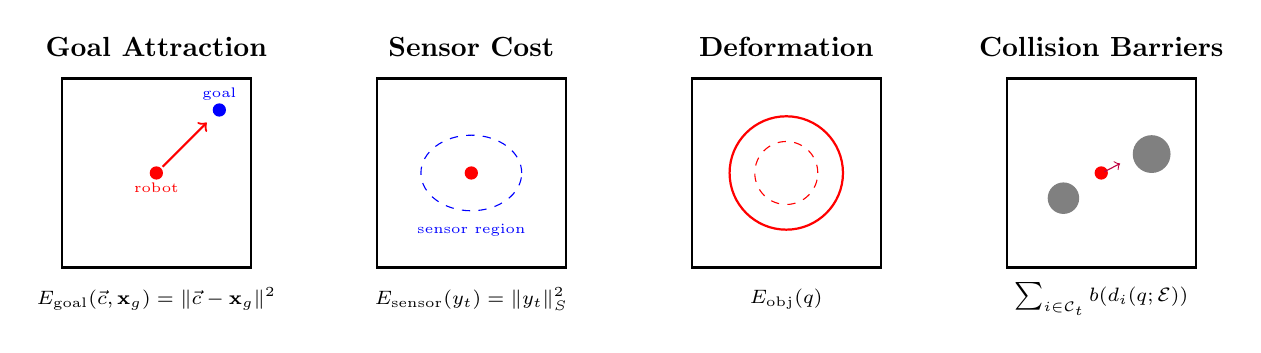
\begin{tikzpicture}[scale=0.8]

% Goal Attraction (Frame Policy)
\begin{scope}[shift={(-7.5,2)}]
    \draw[thick] (-1.5,-1.5) rectangle (1.5,1.5);
    \node[above] at (0,1.7) {\textbf{Goal Attraction}};
    \fill[red] (0,0) circle (3pt) node[below] {\tiny robot};
    \fill[blue] (1,1) circle (3pt) node[above] {\tiny goal};
    \draw[->,thick,red] (0.1,0.1) -- (0.8,0.8);
    \node at (0,-2) {\scriptsize $E_{\mathrm{goal}}(\vec{c},\mathbf{x}_g) = \|\vec{c}-\mathbf{x}_g\|^2$};
\end{scope}

% Sensor Cost (Sensor Policy)
\begin{scope}[shift={(-2.5,2)}]
    \draw[thick] (-1.5,-1.5) rectangle (1.5,1.5);
    \node[above] at (0,1.7) {\textbf{Sensor Cost}};
    \fill[red] (0,0) circle (3pt);
    \draw[blue,dashed] (0,0) ellipse (0.8 and 0.6);
    \node[blue] at (0,-0.9) {\tiny sensor region};
    \node at (0,-2) {\scriptsize $E_{\mathrm{sensor}}(y_t)=\|y_t\|_{S}^2$};
\end{scope}

% Deformation (Shape Policy)
\begin{scope}[shift={(2.5,2)}]
    \draw[thick] (-1.5,-1.5) rectangle (1.5,1.5);
    \node[above] at (0,1.7) {\textbf{Deformation}};
    \draw[red,thick] (0,0) circle (0.9);   % expanded radius
    \draw[red,dashed] (0,0) circle (0.5); % contracted radius
    \node at (0,-2) {\scriptsize $E_{\mathrm{obj}}(q)$};
\end{scope}

% Collision Barriers
\begin{scope}[shift={(7.5,2)}]
    \draw[thick] (-1.5,-1.5) rectangle (1.5,1.5);
    \node[above] at (0,1.7) {\textbf{Collision Barriers}};
    \fill[red] (0,0) circle (3pt);
    \fill[gray] (0.8,0.3) circle (0.3);
    \fill[gray] (-0.6,-0.4) circle (0.25);
    \draw[->,purple] (0.05,0.02) -- (0.3,0.15);
    \node at (0,-2) {\scriptsize $\sum_{i\in\mathcal{C}_t} b(d_i(q;\mathcal{E}))$};
\end{scope}

\end{tikzpicture}
\caption{
Policy-aligned energy decomposition in GRL--SNAM.
The sensor policy exposes a sensor configuration cost $E_{\mathrm{sensor}}$, 
the frame policy induces goal attraction $E_{\mathrm{goal}}$, 
and the shape policy contributes deformation energy $E_{\mathrm{obj}}$, 
while all modules share collision barrier terms $b(d_i)$ around active constraints $\mathcal{C}_t$.
A meta-policy $g_\xi$ assigns weights $(\beta,\lambda,\{\alpha_i\})$ to these components to form the surrogate potential
$\mathcal{R}(q;\eta_\xi^t,\mathcal{E}) = E_{\mathrm{sensor}} + \beta^t E_{\mathrm{goal}} + \lambda^t E_{\mathrm{obj}} + \sum_{i\in\mathcal{C}_t} \alpha_i^t b(d_i)$
used in the Hamiltonian dynamics.
}
\label{fig:energy_decomposition}
\end{figure}
% =======================================================================
\section{Three-Module Architecture and Multi-Scale Coordination}
\label{sec:ch3:architecture}
% =======================================================================

\subsection{Policy Decomposition across Timescales}
\label{subsec:ch3:decomp}

GRL-SNAM treats the SNAM problem as finding three sub-policies operating
at different effective timescales, realised by decomposing $H$ into three
Hamiltonians:
\begin{equation}
  H = H_y(T^*\mathcal{Q}_y) \;+\; H_f(T^*\mathcal{Q}_f)
      \;+\; H_o(T^*\mathcal{Q}_o),
  \label{eq:ch3:ham_decomp}
\end{equation}
with corresponding policies:
\begin{enumerate}
  \item \textbf{Sensing policy} $\pi_y : T^*\mathcal{Q}_y \to T^*\mathcal{Q}_y$
        — updates sensor configuration $\vec{y}$ to acquire local obstacle
        context; fires every $T_y$ steps.
  \item \textbf{Frame policy} $\pi_f : T^*\mathcal{Q}_f \to T^*\mathcal{Q}_f$
        — plans short-horizon motion in $\vec{c}$-space toward the stage
        exit goal; fires every $T_f$ steps.
  \item \textbf{Shape policy} $\pi_o : T^*\mathcal{Q}_o \to T^*\mathcal{Q}_o$
        — modulates morphology $\vec{\psi}$ (deformation scale) to exploit
        narrow passages; fires every $T_o$ steps.
\end{enumerate}
Rather than stacking these as a manually tuned hierarchy, each sub-policy
is the flow map of its own energy terms under a shared environment
codex.
Temporal scale separation emerges from the different periods
$(T_y, T_f, T_o)$, not from hand-designed reward decompositions.

\subsection{The Meta-Navigator: Context to Energy}
\label{subsec:ch3:metanav}

All three sub-policies are parameterized by a shared meta-navigator
$g_\xi$ that maps each local context $\mathcal{E}_\tau$ to a full
Hamiltonian specification:
\begin{equation}
  g_\xi : \mathcal{E}_\tau
  \longmapsto
  \bigl\{
    H_y(\cdot;\mathcal{E}_\tau),\;
    H_f(\cdot;\mathcal{E}_\tau),\;
    H_o(\cdot;\mathcal{E}_\tau)
  \bigr\},
  \label{eq:ch3:metanav}
\end{equation}
or equivalently, to the coefficient vector
$(\beta^t, \lambda^t, \{u_{f}^{\xi,t}\}, \{\mu_f^{\xi,t}\}, \{\alpha_i^t\})$
that instantiates the potential \cref{eq:ch3:potential}.
The parameter set $\xi$ is learned offline and then applied online
without further gradient computation at inference time. Figure~\ref{fig:independent-score-architecture} shows the complete pipeline from context to multi-scale flow maps.

\begin{figure}[htbp]
\centering
\resizebox{\linewidth}{!}{%
\begin{tikzpicture}[
  node distance=0.5cm,
  font=\small,
  % --- Colors ---
  sensorcolor/.style={draw=RoyalBlue, fill=RoyalBlue!10},
  framecolor/.style ={draw=Crimson,   fill=Crimson!10},
  shapecolor/.style ={draw=ForestGreen,fill=ForestGreen!10},
  navcolor/.style   ={draw=Orange,    fill=Orange!10},
  band/.style       ={fill=black!3, draw=none},
  % --- Styles ---
  mod/.style   ={rectangle,rounded corners=2pt,draw,very thick,align=center,
                 minimum width=4.8cm,minimum height=2.2cm,#1},
  nav/.style   ={rectangle,rounded corners=2pt,draw,very thick,align=center,
                 minimum width=14.0cm,minimum height=2.0cm,#1},
  io/.style    ={circle,draw,thick,inner sep=0pt,minimum size=2.8mm,fill=white},
  qarr/.style  ={thick,dashed,-{Stealth[length=2.2mm]}},
  rarr/.style  ={thick,-{Stealth[length=2.2mm]}},
  chip/.style  ={rectangle,rounded corners=1pt,draw,thin,inner sep=2pt,
                 font=\scriptsize,fill=white},
  dsicon/.style={rectangle,draw,thin,fill=white,minimum width=4.5mm,minimum height=4.5mm},
  badge/.style ={circle,draw,thin,fill=white,minimum size=5mm,font=\scriptsize\bfseries},
  xtiny/.style ={font=\scriptsize},
  response/.style={rectangle,draw,thin,fill=white,rounded corners=1pt,font=\scriptsize,align=left,inner sep=3pt}
]

% ====== GRID COORDS ======
\coordinate (ColY) at (-5.2,0);   % Sensor column x
\coordinate (ColF) at ( 0.0,0);   % Frame column x
\coordinate (ColO) at ( 5.2,0);   % Shape column x

% ====== Background band ======
\node[rectangle,band,minimum width=16.5cm,minimum height=2.8cm,anchor=center] at (0,6.0) {};

% ====== MODULES (moved up) ======
% Sensor module
\node[mod=sensorcolor,anchor=center] (sensor) at ($(ColY)+(0,6.0)$) {
    {\bfseries\color{RoyalBlue}Sensor Policy $\pi_y^{\theta_y,\xi}$}\\[2pt]
    {\scriptsize $s_y^{\theta_y,\xi}(z_y,t;\mathcal{E})=\mathbb{J}\nabla_{z_y}h_y^{\theta_y}$}\\[1pt]
    {\scriptsize\color{gray} $\Gamma_y^\xi\equiv 0,\; G_y^\xi u_y^\xi\equiv 0$}
};

% Frame module
\node[mod=framecolor,anchor=center] (frame) at ($(ColF)+(0,6.0)$) {
    {\bfseries\color{Crimson}Frame Policy $\pi_f^{\theta_f,\xi}$}\\[1pt]
    {\scriptsize $s_f^{\theta_f,\xi}=\mathbb{J}\nabla_{z_f}h_f^{\theta_f}+\begin{bmatrix}0\\-\Gamma_f^\xi\dot{q}_f+G_f^\xi u_f^\xi\end{bmatrix}$}\\[1pt]
    {\scriptsize\color{gray} $\Gamma_f^\xi=\mu_\xi(\mathcal{E})\mathbf{I},\; G_f^\xi=\mathbf{I}$}
};

% Shape module
\node[mod=shapecolor,anchor=center] (shape) at ($(ColO)+(0,6.0)$) {
    {\bfseries\color{ForestGreen}Shape Policy $\pi_o^{\theta_o,\xi}$}\\[2pt]
    {\scriptsize $s_o^{\theta_o,\xi}(z_o,t;\mathcal{E})=\mathbb{J}\nabla_{z_o}h_o^{\theta_o}$}\\[1pt]
    {\scriptsize\color{gray} $\Gamma_o^\xi\equiv 0,\; G_o^\xi u_o^\xi\equiv 0$}
};

% ====== Configuration space icons (top-left inside each) ======
\foreach \M/\L in {sensor/$\mathcal{Q}_y$,frame/$\mathcal{Q}_f$,shape/$\mathcal{Q}_o$}{
  \node[dsicon] (ds-\M) at ([xshift=4mm,yshift=-3mm]\M.north west) {};
  \draw[thin] (ds-\M.south west)++(0,0.6mm) rectangle ++(4.5mm,0.8mm);
  \draw[thin] (ds-\M.south west)++(0,1.8mm) rectangle ++(4.5mm,0.8mm);
  \draw[thin] (ds-\M.south west)++(0,3.0mm) rectangle ++(4.5mm,0.8mm);
  \node[xtiny] at ([xshift=7mm]ds-\M.east) {\L};
}

% ====== Time badges (outside top-right) ======
\node[badge,text=RoyalBlue]   at ([xshift=-14pt,yshift=8pt]sensor.north east) {$T_y$};
\node[badge,text=Crimson]     at ([xshift=-14pt,yshift=8pt]frame.north east)  {$T_f$};
\node[badge,text=ForestGreen] at ([xshift=-14pt,yshift=8pt]shape.north east)  {$T_o$};

% ====== Timescale annotation ======
\node[xtiny,anchor=west] at (8.0,7.6) {$T_y \gg T_f \gg T_o$};

% ====== POTENTIAL TERMS (above modules) ======
\node[chip,fill=RoyalBlue!5] at ([yshift=6pt]sensor.north) {$\mathcal{R}_y: E_{\mathrm{sensor}} + \sum_i\alpha_i b(d_i)$};
\node[chip,fill=Crimson!5] at ([yshift=6pt]frame.north) {$\mathcal{R}_f: \beta E_{\mathrm{goal}} + \sum_i\alpha_i b(d_i)$};
\node[chip,fill=ForestGreen!5] at ([yshift=6pt]shape.north) {$\mathcal{R}_o: \lambda E_{\mathrm{obj}} + \sum_i\alpha_i b(d_i)$};

% ====== RESPONSE BOXES (between modules and navigator) ======
\node[response,fill=RoyalBlue!5] (Ry) at ($(ColY)+(0,3.6)$) {
    $\mathsf{R}_y=\big\{z_{0:T_y}^{(y)},\mathrm{QoI}_y\big\}$\\
    $\mathrm{QoI}_y=\Delta\mathcal{E}$
};
\node[response,fill=Crimson!5] (Rf) at ($(ColF)+(0,3.6)$) {
    $\mathsf{R}_f=\big\{z_{0:T_f}^{(f)},\mathrm{QoI}_f\big\}$\\
    $\mathrm{QoI}_f=\{v_t^{(f)}\}_{t=0}^{T_f}$
};
\node[response,fill=ForestGreen!5] (Ro) at ($(ColO)+(0,3.6)$) {
    $\mathsf{R}_o=\big\{z_{0:T_o}^{(o)},\mathrm{QoI}_o\big\}$\\
    $\mathrm{QoI}_o=\{\min_i d_i\}_{t=0}^{T_o}$
};

% ====== NAVIGATOR ======
\node[nav=navcolor,anchor=center] (nav) at ($(0,1.2)$) {
  {\bfseries Navigator $g_{\xi}$ (Meta-Hamiltonian Composer)}\\[2pt]
  {\scriptsize Tokenize: $\mathcal{T}_t=\mathrm{Tokenize}(\mathcal{C}_t(\mathcal{E},q_t),\,q_t,\,\mathbf{x}_g)$\quad\quad Output: $g_\xi(\mathcal{E})=\big[\,\eta_\xi,\;\mu_\xi,\;u_f^\xi\,\big]$}\\[1pt]
  {\scriptsize Dual weights: $\eta_\xi(\mathcal{E})=(\beta,\lambda,\{\alpha_i\}_{i\in\mathcal{C}_t})$\quad\quad Surrogate: $H=\tfrac{1}{2}p^{\top}M^{-1}p+\mathcal{R}(q;\eta_\xi,\mathcal{E})$}
};

% ====== QUERY ARROWS (Navigator to Modules) ======
\draw[qarr,draw=RoyalBlue]
  ([xshift=-8pt]nav.north-|ColY) -- node[xtiny,fill=white,inner sep=1pt,pos=0.5,left]
  {$(H_y,z_y^t,T_y)$} ([xshift=-8pt]Ry.south-|ColY);

\draw[qarr,draw=Crimson]
  ([xshift=-8pt]nav.north-|ColF) -- node[xtiny,fill=white,inner sep=1pt,pos=0.5,left]
  {$(H_f,z_f^t,T_f,\Gamma_f^\xi,u_f^\xi)$} ([xshift=-8pt]Rf.south-|ColF);

\draw[qarr,draw=ForestGreen]
  ([xshift=-8pt]nav.north-|ColO) -- node[xtiny,fill=white,inner sep=1pt,pos=0.5,left]
  {$(H_o,z_o^t,T_o)$} ([xshift=-8pt]Ro.south-|ColO);

% ====== RESPONSE ARROWS (Response boxes to Navigator) ======
\draw[rarr,draw=RoyalBlue]
  ([xshift=8pt]Ry.south-|ColY) -- ([xshift=8pt]nav.north-|ColY);

\draw[rarr,draw=Crimson]
  ([xshift=8pt]Rf.south-|ColF) -- ([xshift=8pt]nav.north-|ColF);

\draw[rarr,draw=ForestGreen]
  ([xshift=8pt]Ro.south-|ColO) -- ([xshift=8pt]nav.north-|ColO);

% ====== ARROWS from Modules to Response boxes ======
\draw[rarr,draw=RoyalBlue] (sensor.south) -- (Ry.north);
\draw[rarr,draw=Crimson] (frame.south) -- (Rf.north);
\draw[rarr,draw=ForestGreen] (shape.south) -- (Ro.north);

% ====== Environment & Trajectory ======
\node[rectangle,draw,thick,fill=white,minimum width=2.6cm,minimum height=1.0cm,align=center]
      (env) at (-9.2,1.2) {{\bfseries Environment $\mathcal{E}$}\\ {\scriptsize $z_0,\;\mathbf{x}_g,\;\{d_i\geq 0\}$}};
\node[rectangle,draw,thick,fill=white,minimum width=2.6cm,minimum height=1.0cm,align=center]
      (traj) at ( 9.2,1.2) {{\bfseries Trajectory}\\ {\scriptsize $\{z_t\}_{t=0}^{T}$}};

\draw[thick,-{Stealth[length=2.5mm]}] (env.east) -- (nav.west);
\draw[thick,-{Stealth[length=2.5mm]}] (nav.east) -- (traj.west);

% ====== Side annotations ======
% Symplectic matrix definition (left)
\node[rectangle,draw,thin,fill=white,align=left,font=\scriptsize,inner sep=4pt]
      at (-9.8,5.8) {
       \textbf{Symplectic form:}\\[1pt]
       $\mathbb{J}=\begin{bmatrix}0 & I\\-I & 0\end{bmatrix}$\\[1pt]
       $\mathbb{J}\nabla_z h = \begin{bmatrix}\nabla_p h\\-\nabla_q h\end{bmatrix}$
      };

% Online adaptation (right)
\node[rectangle,draw,thin,fill=white,align=left,font=\scriptsize,inner sep=4pt]
      at (10.5,5.8) {
       \textbf{Online observables:}\\[1pt]
       $y_t=[-\mathrm{clr}_t,\mathrm{dist}_t,-\mathrm{speed}_t]^\top$\\[1pt]
       Adapt $\zeta_t=[\eta_t,\mu_t]$ via $J_t\approx\partial y/\partial\zeta$
      };

% ====== Compact Legend ======
\node[rectangle,draw,thick,fill=white,align=left,font=\scriptsize,inner sep=4pt]
      at (0,-0.8) {
       \textbf{Legend:}\;
       \tikz[baseline=-0.5ex]{\node[io]{};} port\quad
       \tikz[baseline=-0.5ex]{\draw[qarr] (0,0)--(8mm,0);} query\quad
       \tikz[baseline=-0.5ex]{\draw[rarr] (0,0)--(8mm,0);} response
       \qquad
       \textbf{Policy as flow:}\; $\pi_k^{\theta_k,\xi}(\mathcal{E}):=\Phi_k^{\Delta t}(\cdot;\mathcal{E})$
      };

\end{tikzpicture}}
\caption{%
Modular score-field architecture for GRL-SNAM.
The Navigator $g_\xi$ tokenizes active constraints $\mathcal{C}_t$, state $q_t$, and goal $\mathbf{x}_g$, then outputs dual weights $\eta_\xi=(\beta,\lambda,\{\alpha_i\})$, friction $\mu_\xi$, and port correction $u_f^\xi$.
Each module $k\in\{y,f,o\}$ integrates its score field $s_k^{\theta_k,\xi}=\mathbb{J}\nabla_{z_k}h_k^{\theta_k}$ (plus non-conservative terms for the frame module) over horizon $T_k$ and returns response $\mathsf{R}_k$ with phase-space rollouts and QoIs.
The frame module uniquely receives dissipation $\Gamma_f^\xi$ and port input $u_f^\xi$; sensor and shape modules have purely symplectic dynamics.
}
\label{fig:independent-score-architecture}
\end{figure}


% =======================================================================
\section{Learning and Online Correction}
\label{sec:ch3:learning}
% =======================================================================

\subsection{Offline Meta-Training}
\label{subsec:ch3:offline}

During offline training, GRL-SNAM learns $\xi$ (the parameters of $g_\xi$)
from a dataset of trajectory-context pairs $\{(\vec{q}_{0:T}, \mathcal{E})\}$
collected across diverse procedurally generated environments.
The training loss combines four terms:
\begin{equation}
  \mathcal{L}(\xi)
  = w_{\mathrm{traj}}\,\mathcal{L}_{\mathrm{traj}}
  + w_{\mathrm{vel}}\,\mathcal{L}_{\mathrm{vel}}
  + w_{\mathrm{fric}}\,\mathcal{L}_{\mathrm{fric}}
  + w_{\mathrm{multi}}\,\mathcal{L}_{\mathrm{multi}},
  \label{eq:ch3:loss}
\end{equation}
where:
\begin{itemize}
  \item $\mathcal{L}_{\mathrm{traj}} = \sum_t \|\vec{q}_t^{\mathrm{pred}}
        - \vec{q}_t^{\mathrm{ref}}\|^2$ supervises trajectory matching
        against reference rollouts from short Hamiltonian integrations;
  \item $\mathcal{L}_{\mathrm{vel}} = \sum_t \|\dot{\vec{q}}_t^{\mathrm{pred}}
        - \dot{\vec{q}}_t^{\mathrm{ref}}\|^2$ supervises velocity matching;
  \item $\mathcal{L}_{\mathrm{fric}} = \|\gamma - \gamma_{\mathrm{ref}}\|^2$
        aligns the learned dissipation coefficient with a stagewise
        reference, preventing under-damped oscillation in the barrier
        channels;
  \item $\mathcal{L}_{\mathrm{multi}}$ trains near-contact robustness via
        perturbed short rollouts sampled from multiple start configurations
        close to constraint boundaries.
\end{itemize}
The design of $\mathcal{L}_{\mathrm{fric}}$ is motivated by the
port-Hamiltonian passivity condition (Definition~\ref{def:passivity}):
learning an appropriate dissipation term ensures that energy is not
spuriously injected when the Hamiltonian is updated.

\subsection{Online Geometric Alignment}
\label{subsec:ch3:online}

At test time the agent encounters environments not seen during training.
Rather than relearning $\xi$ from scratch, GRL-SNAM performs
\emph{online geometric alignment}: the meta-navigator $g_\xi$ (fixed)
maps each new context $\mathcal{E}_\tau$ to a Hamiltonian, and a
lightweight correction signal $u_f^{\xi,t}$ is computed from recent
rollout feedback to update the barrier weights:
\begin{equation}
  \alpha_i^{t+1}
  = \alpha_i^t
    + \eta_\alpha\,\frac{\partial \mathcal{L}_{\mathrm{safe}}}
                        {\partial \alpha_i}\Bigg|_{z_t},
  \label{eq:ch3:online_update}
\end{equation}
where $\mathcal{L}_{\mathrm{safe}}$ penalizes clearance violations
observed in the current rollout.
This update reshapes only the barrier weights—not the full parameter
set $\xi$—so it is fast, stable, and non-destructive of the offline
learned structure.

The online correction loop follows the segment-level timescale of
Figure~\ref{fig:prelim:timescales}: after each navigation segment,
$\{\alpha_i^t\}$ are updated before the next stage begins.

\subsection{Online Pipeline}
\label{subsec:ch3:pipeline}

\begin{algorithm}[htbp]
\caption{Online GRL-SNAM pipeline}
\label{algo:online_grl_snam_main:short}
\begin{algorithmic}[1]
\State \textbf{Input:} goal $\mathbf{x}_g$, initial $z_0=(q_0,p_0)$ (typically $p_0{=}0$), step $\tau$, horizons $(T_y,T_f,T_o)$, max steps $N_{\max}$
\State \textbf{Init:} $n\!\leftarrow\!0$, environment $\mathcal{E}_0$, environment counter $\tau\gets 0$ active set $\mathcal{C}_0\!\leftarrow\!\emptyset$
\State \textbf{Init:} meta state $(\eta_0,\mu_0,u_{f,0})$ from network $g_\xi$,
\State Assemble $H$ by computing $g_{\xi}(\mathcal{E}_{0})$
\While{$\neg$\textsc{ReachedGoal}$(\vec{c}_n,\mathbf{x}_g)$ \textbf{and} $n<N_{\max}$}
    
    \If{$n \equiv 0 \pmod{T_y}$}   
        \State Assemble $H_y$, provide $z_{y,0}$.
        \State Query Sensor Process via $\pi_y$ and get response $\mathsf{R}_y$
    \EndIf
    \If{$n \equiv 0 \pmod{T_f}$}
        \State Assemble $H_f$, $u_{f}^{\xi,n}, \mu_{f}^{\xi,n}$, provide $z_{f,0}$.
        \State Query Free Path Extractor via $\pi_f$ and get response $\mathsf{R}_f$
    \EndIf
    \If{$n \equiv 0 \pmod{T_o}$}
        \State Assemble $H_o$, provide $z_{o,0}$.
        \State Query Shape Reconfig via $\pi_o$ and get response $\mathsf{R}_o$
    \EndIf
    \State Collect QoIs $y_n$ from responses $\mathsf{R}_y$, $\mathsf{R}_f$ and $\mathsf{R}_o$.
    \State Compute correction term $u_f^{\xi,n}$ via $y_n$.
    \If{$n \equiv 0 \pmod{T_y}$ \textbf{or} reach stage goal}
    \State Update $\mathcal{E}_{\tau+1}$ via response $\mathsf{R}_y$.
    \State Reassemble $H$ by computing $g_{\xi}(\mathcal{E}_{\tau+1})$
    \State $\tau\gets \tau+1$
    \EndIf
    \State $n\leftarrow n+1$
\EndWhile
\State \textbf{Return:} trajectory $\{z_n\}_{n=0}^{N}$ and parameter history $\{(\eta_n,\mu_{f}^{\xi,n},u_{f}^{\xi,n})\}_{n=0}^{N}$
\end{algorithmic}
\end{algorithm}

Algorithm~\ref{algo:online_grl_snam_main:short} shows the complete
online pipeline, reused from the GRL-SNAM paper.
The outer while loop advances stage index $\tau$ each time the
sensing policy detects a new context or a stage goal is reached.
Within each stage, the three sub-policies fire at their respective
periods, collecting responses $\mathsf{R}_y, \mathsf{R}_f, \mathsf{R}_o$
that supply the correction signal $u_f^{\xi,t}$.

% \input{tex/alg0_overall_loop}

% =======================================================================
\section{Experimental Evaluation}
\label{sec:ch3:experiments}
% =======================================================================

\subsection{Tasks and Environments}
\label{subsec:ch3:tasks}

We evaluate GRL-SNAM on two benchmarks sharing the same
stagewise local-sensing interface.

\paragraph{Hyperelastic ring navigation.}
The primary benchmark is a deformable hyperelastic ring robot navigating
through cluttered workspaces with narrow passages, bottlenecks, and
zig-zag corridors.
Start–goal pairs are sampled so that the deformable ring admits a
collision-free solution, while a rigid disc of comparable size may not.
Train, in-distribution (\textbf{Test-ID}), and out-of-distribution
(\textbf{Test-OOD}, shifted gap/density) splits are constructed.
All baselines use the same stage manager and local sensing window as
GRL-SNAM.

\paragraph{Dungeon point-agent navigation.}
The secondary benchmark uses dungeon layouts
with a point-mass agent in continuous 2D.
A \texttt{StagewiseSensor} provides the active stage exit; an
\texttt{ObstacleExtractor} fits circular obstacles to locally visible
wall segments.
This benchmark isolates the learning formulation from deformability.

\subsection{Baselines}
\label{subsec:ch3:baselines}

We compare against:
\begin{itemize}
  \item \textbf{Global planners (full map):} Rigid A$^*$ and
        Deformable A$^*$ using full occupancy grids as references.
  \item \textbf{Reactive local planners (same sensing):} Potential
        Fields (PF), Control Barrier Functions (CBF), and Dynamic
        Window Approach (DWA), all operating under the same stagewise
        local window.
  \item \textbf{Deep RL baselines:} PPO~\citep{schulman2017proximalpolicyoptimizationalgorithms},
        TRPO~\citep{schulman2017trustregionpolicyoptimization}, and
        SAC~\citep{haarnoja2018softactorcriticoffpolicymaximum} under both full-episode and
        stagewise short-rollout regimes.
  \item \textbf{Within-framework ablations:} velocity regression and
        coefficient RL, replacing Hamiltonian-structured supervision
        with flat alternatives on the same dataset.
\end{itemize}

\subsection{Results}
\label{subsec:ch3:results}

\paragraph{Hyperelastic ring: navigation quality.}
Table~\ref{tab:ch3:ring} summarizes the main results on the ring
benchmark.
GRL-SNAM achieves the highest success rate on both Test-ID and
Test-OOD splits, with the lowest collision count and best
success-weighted path length (SPL).
Crucially, it achieves near-planner efficiency while using only local
sensing ($\rho_{\mathrm{map}} < 0.35$ on all splits), compared to the
global A$^*$ reference that requires the full map.

\begin{table}[t]
\centering
\caption{%
  \textbf{Navigation results on the hyperelastic ring benchmark.}
  GRL-SNAM achieves competitive navigation quality using only local
  sensing; global planners are upper-bound references with full map
  access.
  $\uparrow$/$\downarrow$ denote desired direction.
}
\label{tab:ch3:ring}
\small
\setlength{\tabcolsep}{5pt}
\renewcommand{\arraystretch}{1.2}
\begin{tabular}{lcccccc}
\toprule
\textbf{Method} & \textbf{Map} &
\makecell{\textbf{Success}\\\textbf{(\%)}$\uparrow$} &
\makecell{\textbf{SPL}$\uparrow$} &
\makecell{\textbf{MinClr}\\(m)$\uparrow$} &
\makecell{\textbf{Collisions}$\downarrow$} &
\makecell{$\rho_{\mathrm{map}}\downarrow$} \\
\midrule
Rigid A$^*$        & Full & 78.4  & 0.91 & 0.31 & 0.2 & 1.00 \\
Deformable A$^*$   & Full & 94.1  & 0.88 & 0.28 & 0.1 & 1.00 \\
\midrule
PF (staged)        & Local & 51.3 & 0.61 & 0.14 & 3.8 & 0.31 \\
CBF (staged)       & Local & 63.7 & 0.68 & 0.22 & 1.2 & 0.29 \\
DWA (staged)       & Local & 58.2 & 0.65 & 0.19 & 2.1 & 0.32 \\
\midrule
\textbf{GRL-SNAM (Test-ID)}  & Local & \textbf{98.7} & \textbf{0.82} & \textbf{0.36} & \textbf{0.3} & \textbf{0.33} \\
\textbf{GRL-SNAM (Test-OOD)} & Local & \textbf{91.5} & \textbf{0.76} & 0.31 & 0.6 & 0.35 \\
\bottomrule
\end{tabular}
\end{table}

\paragraph{Dungeon navigation: objective dominates optimizer.}
Table~\ref{tab:ch3:dungeon} reports dungeon results under the stagewise
interface.
Full-episode RL (Table~\ref{tab:ch3:full_rl}) fails substantially, with
PPO achieving only 7.2\% success after 5M steps.
Stagewise short-rollout RL improves but plateaus at 18–26\%.
GRL-SNAM with Hamiltonian-structured supervision achieves 87.5\% success
at 500k gradient steps.
The consistent gap between RL and GRL-SNAM with the \emph{same}
observation/action interface isolates the advantage: it comes from
structured supervision, not from richer observations.

\begin{table}[t]
\centering
\caption{%
  \textbf{Dungeon navigation: stagewise short-rollout comparison.}
  All methods share the same stagewise interface, sensors, and encoder.
  GRL-SNAM achieves 87.5\% success vs.\ 18--26\% for RL baselines,
  demonstrating that the learning formulation—not the action space or
  encoder—drives the performance gap.
}
\label{tab:ch3:dungeon}
\small
\setlength{\tabcolsep}{6pt}
\renewcommand{\arraystretch}{1.2}
\begin{tabular}{lcccc}
\toprule
\textbf{Method} &
\makecell{\textbf{Success}\\\textbf{(\%)}$\uparrow$} &
\makecell{\textbf{State error}\\\textbf{(m)}$\downarrow$} &
\makecell{\textbf{Goal dist.}\\\textbf{(m)}$\downarrow$} &
\textbf{Steps} \\
\midrule
PPO      & 26.1 & 1.8 & 1.2 & $\approx$3.2M \\
TRPO     & 21.7 & 2.1 & 1.5 & $\approx$3.8M \\
SAC      & 18.4 & 2.4 & 1.9 & $\approx$4.1M \\
\midrule
\textbf{GRL-SNAM} & \textbf{87.5} & \textbf{0.3} & \textbf{0.1} & 500k \\
\bottomrule
\end{tabular}
\end{table}

\begin{table}[t]
\centering
\caption{%
  \textbf{Full-episode RL baselines.}
  Standard end-to-end RL without stagewise structure fails substantially
  in the dungeon task.
}
\label{tab:ch3:full_rl}
\small
\setlength{\tabcolsep}{6pt}
\renewcommand{\arraystretch}{1.2}
\begin{tabular}{lcccc}
\toprule
\textbf{Method} & \textbf{Success (\%)} &
\textbf{Goal dist.\ (m)} & \textbf{Collision (\%)} & \textbf{Steps} \\
\midrule
PPO  & 7.2  & 14.1 & 23.5 & 5M \\
TRPO & 3.8  & 23.7 & 26.1 & 6.5M \\
SAC  & 1.5  & 20.2 & 28.3 & 8M \\
\bottomrule
\end{tabular}
\end{table}

\begin{figure}[htbp]
    \centering
    \includegraphics[width=0.55\textwidth]{barrier_radial_profile.png}
    \caption{\textbf{Radial profile of barrier energy vs.\ clearance.}
    Angle-averaged barrier energy around obstacles for the learned barrier (solid) and analytic reference (dashed).
    The learned profile matches the reference trend and sharpens near contact. { The difference between two curves indicates Our method can learn to adapt the energy landscape based on its current environment context.}}
    \label{fig:barrier_profile}
\end{figure}

\paragraph{Hamiltonian field analysis.}
Figures~\ref{fig:vector_fields} and~\ref{fig:time_series} reveal the
qualitative behavior of the learned field.
The force decomposition $F = \beta F_g + \gamma F_{\mathrm{bs}}$ produces
smooth, clearance-preserving arcs around clutter through context-dependent
coefficient reweighting.
Along a representative rollout, the coefficients $(\beta,\gamma,\alpha)$
adapt smoothly as the robot enters and exits tight passages—not through
ad-hoc action scaling, but through Hamiltonian reparameterization.
The learned barrier profile (Figure~\ref{fig:barrier_profile}) closely
tracks the analytic reference while capturing additional material
softening at intermediate distances.

\begin{figure}[htbp]
    \centering
\includegraphics[width=0.8\textwidth]{vector_fields_example.png}
\caption{\textbf{Learned Hamiltonian field decomposition.}
Shown are the constituent fields used by GRL-SNAM to generate local motion under partial, stagewise observations.
\textbf{Left:} $F_g$ points toward the current stage goal and captures progress, but ignores obstacles.
\textbf{Middle:} $F_{bs}$ is induced by locally sensed barriers and encodes avoidance/clearance, but lacks task direction.
\textbf{Right:} the deployed field $F=\beta F_g+\gamma F_{bs}$ combines both effects; the learned, context-dependent coefficients $(\beta,\gamma)$ modulate the relative strength of goal following vs.\ obstacle avoidance, producing a trajectory direction that threads the corridor while maintaining a safety margin near contact regions.}
\label{fig:vector_fields}
\end{figure}

\begin{figure}[htbp]
    \centering
    \includegraphics[width=0.6\textwidth]{timeseries_forces_clearance_coeffs.png}
    \caption{\textbf{Temporal analysis of Hamiltonian adaptation.}
    Top: minimum clearance. Middle: $|F_g|$ and $|F_{bs}|$. Bottom: coefficients $(\beta,\gamma,\alpha)$.
    Coefficients change smoothly as the robot enters/exits clutter, rebalancing goal and barrier terms.}
    \label{fig:time_series}
\end{figure}

\paragraph{Robustness.}
Table~\ref{tab:ch3:robustness} shows that GRL-SNAM maintains
$\geq 87\%$ success under severe sensing and dynamics perturbations
(position jitter, obstacle hallucination, damping mismatch).
Rather than failing catastrophically under constraint mis-specification,
the learned Hamiltonian re-weights goal and barrier terms from the
distorted local observations, preserving a meaningful
safety–progress trade-off.

\begin{table}[t]
\centering
\caption{%
  \textbf{Robustness to sensing and dynamics perturbations.}
  GRL-SNAM degrades gracefully—87\% success even under severe noise—
  because adaptation operates through energy-coefficient reshaping,
  not overfitting to a nominal model.
}
\label{tab:ch3:robustness}
\small
\setlength{\tabcolsep}{6pt}
\renewcommand{\arraystretch}{1.2}
\begin{tabular}{lcccc}
\toprule
\textbf{Perturbation} &
\makecell{\textbf{Success}\\\textbf{(\%)}$\uparrow$} &
\textbf{SPL}$\uparrow$ &
\makecell{\textbf{Min.\ Clr}\\\textbf{(m)}$\uparrow$} &
\textbf{Collisions}$\downarrow$ \\
\midrule
Nominal (0.0, 1.0)        & 98.7 & 0.82 & 0.36 & 0.3 \\
Mild noise (0.05, 0.9)    & 91.3 & 0.79 & 0.33 & 0.7 \\
Severe noise (0.10, 0.7)  & 87.1 & 0.72 & 0.29 & 1.1 \\
\bottomrule
\end{tabular}
\end{table}

\paragraph{Ablation: loss components.}
Table~\ref{tab:ch3:ablation} isolates the contributions of the
friction and multi-start loss terms.
Without $\mathcal{L}_{\mathrm{fric}}$, the field is under-damped and
oscillatory, producing barrier violations; without
$\mathcal{L}_{\mathrm{multi}}$, the field is overly conservative.
Both terms play distinct interpretable roles: friction learns appropriate
dissipation (port-Hamiltonian passivity), while multi-start shapes the
field near constraint boundaries.

\begin{table}[t]
\centering
\caption{%
  \textbf{Ablation of training loss components.}
  The friction loss $\mathcal{L}_{\mathrm{fric}}$ is necessary for
  smooth, stable navigation; the multi-start loss
  $\mathcal{L}_{\mathrm{multi}}$ adds robustness near constraints.
}
\label{tab:ch3:ablation}
\small
\setlength{\tabcolsep}{4pt}
\renewcommand{\arraystretch}{1.2}
\begin{tabular}{llccccc}
\toprule
$w_{\mathrm{fric}}$ & $w_{\mathrm{multi}}$ &
\textbf{Collisions}$\downarrow$ &
\textbf{MinClr}$\uparrow$ &
\textbf{Barrier viol.}$\downarrow$ &
\textbf{SPL}$\uparrow$ &
\textbf{Behavior} \\
\midrule
0   & 0   & High & $<0$ & High & Poor & Penetrates obstacles \\
0   & 0.5 & Low  & High & Low  & Low  & Very conservative, slow \\
0.1 & 0   & None & High & Low  & Best & Smooth, stable, fast \\
0.1 & 0.5 & None & High & Low  & High & Robust, tight margins \\
\bottomrule
\end{tabular}
\end{table}

% =======================================================================
\section{What GRL-SNAM Achieves}
\label{sec:ch3:strengths}
% =======================================================================

GRL-SNAM establishes that the geometry-only structured learner provides
a qualitatively different capability from either black-box RL or
classical planners.
The following properties are guaranteed or empirically demonstrated.

\paragraph{Structured field topology.}
The factored potential \cref{eq:ch3:potential} makes the force-field
topology explicit: goal-attracting basins, obstacle-repulsive walls, and
dissipative channels are interpretable, separately modifiable terms.
This contrasts with PPO/SAC policies, where these properties are
hidden in neural weights with no direct handle for structured correction.

\paragraph{Stable online correction.}
The port-Hamiltonian passivity condition (Definition~\ref{def:passivity})
provides a checkable criterion for each adaptation step: as long as
the dissipation matrix $\mathbf{R} \succeq 0$, energy cannot be
spuriously injected.
Online barrier-weight updates \cref{eq:ch3:online_update} satisfy this
criterion by construction.

\paragraph{Minimal sensing effort.}
GRL-SNAM reaches navigation goals with $\rho_{\mathrm{map}} < 0.35$,
meaning it explores less than 35\% of the workspace on average far
below the 100\% required by global planners.
This is a direct consequence of the stagewise local-sensing design:
the agent refines its energy landscape only in the neighborhood it
actually visits.

\paragraph{Sample efficiency.}
500k gradient steps of Hamiltonian-structured supervision suffice to
reach 87.5\% success in the dungeon task an order of magnitude fewer
than the 3–8M environment steps required by RL baselines.
The advantage comes from the learning formulation: structured supervision
over the energy landscape is far more data-efficient than scalar reward
maximization.

\paragraph{Graceful robustness.}
Under severe sensing and dynamics perturbations, GRL-SNAM degrades
gracefully rather than catastrophically, because correction operates
through coefficient reshaping rather than through brittle action-space
memorization.

% =======================================================================
\section{Limitations of Geometry-Only Structure}
\label{sec:ch3:limitations}
% =======================================================================

GRL-SNAM is a powerful geometry-only learner, but three structural
limitations emerge directly from the geometry-only restriction.
These are not implementation failures they are \emph{architectural gaps}
that cannot be closed by tuning the existing framework.

\paragraph{Limitation 1: geometry-blindness to latent material risk.}
The potential \cref{eq:ch3:potential} responds only to signed clearances
$d_i(\vec{q};\mathcal{E})$.
Two regions with identical geometric clearance but different material
properties: one safe grass, one soft mud that immobilizes the robot are
treated identically by GRL-SNAM.
The force field has no channel for material-risk information, because no
such information enters the context $\mathcal{E}_\tau$.

\paragraph{Limitation 2: objective insufficiency for tail-risk behavior.}
The training loss \cref{eq:ch3:loss} optimizes trajectory quality and
clearance margins under an expected-cost criterion.
It cannot optimize the tail distribution of material contact costs—rare
but catastrophic events—because material risk is absent from both the
observation space and the objective.
A geometry-only Hamiltonian has no mechanism for CVaR-type tail-risk
shaping.

\paragraph{Limitation 3: coefficient space too limited for semantic
enrichment.}
The coefficient vector $(\beta, \lambda, \{\alpha_i\})$ in
\cref{eq:ch3:potential} controls only the weights of existing geometric
terms.
Adding a new \emph{type} of force channel: one driven by material
properties rather than signed clearance requires new energy terms,
new coefficients, new gradient pathways, and a new update law.
The geometry-only coefficient space provides no slot for any of these.

\paragraph{Summary.}
These three limitations share a common structure: the geometry-only
learner is constrained by the expressiveness of its energy landscape.
It cannot reason about what it cannot see, and it cannot optimize for
risks it cannot encode.
The missing structure is precisely what Chapter~\ref{chap:material}
introduces: \emph{new energy terms} that carry material-risk and
hazard-barrier information, an \emph{enriched objective} incorporating
CVaR tail-risk, and \emph{new update laws} that operate across the
segment and episode timescales to adapt material-risk coefficients from
experience.

These additions follow the same enrichment principle identified in
Chapter~\ref{chap:hierarchy}: each new energy term induces a new
force channel, a new coefficient, a new objective term, and a new
gradient pathway.
The geometry-only learner does not need to be discarded; it needs to
be enlarged.

% % =======================================================================
% \section{Chapter Summary}
% \label{sec:ch3:summary}
% % =======================================================================

% This chapter established GRL-SNAM as the geometry-only foundation of
% the thesis program.

% The key contributions of this stage are:
% \begin{enumerate}
%   \item A principled derivation of navigation policy as the flow map
%         of a reduced PMP Hamiltonian
%         $H = \frac{1}{2}p^\top\Mass^{-1}p + \Potential(\vec{q};\mathcal{E})$,
%         where the potential decomposes over goal, sensor, shape, and
%         barrier terms (\S\ref{sec:ch3:formulation}).
%   \item A three-module architecture in which sensing, frame, and shape
%         sub-policies are coordinated through a shared energy decomposition
%         at different timescales (\S\ref{sec:ch3:architecture}).
%   \item An offline–online learning scheme in which meta-training learns
%         the context-to-energy mapping $g_\xi$ and online geometric
%         alignment updates barrier coefficients from rollout feedback
%         (\S\ref{sec:ch3:learning}).
%   \item Empirical demonstration that structured Hamiltonian supervision
%         substantially outperforms RL baselines and reactive planners
%         under matched sensing constraints (\S\ref{sec:ch3:experiments}).
% \end{enumerate}

The geometry-only learner is already a continually correctable
navigation policy: its coefficients are updated online, its field
topology is explicit, and its stability is monitored through passivity.
However, it is blind to latent material risk, lacks a tail-risk
objective, and has no energy-coefficient slot for semantic information.

\begin{quote}\itshape
Geometry-only structured Hamiltonian learning yields a principled,
sample-efficient, continually correctable navigation policy under local
sensing but the resulting learner remains blind to latent semantic risk
and therefore motivates the richer material-aware extension of
Chapter~\ref{chap:material}.
\end{quote}